%%%%%%%%%%%%%%%%%%
%  placeholders  %
%%%%%%%%%%%%%%%%%%

\newcommand{\uni}{Technical University of Munich}
\newcommand{\department}{TUM Department of Informatics}
\newcommand{\chair}{Chair for Applied Software Engineering}
\newcommand{\city}{Munich}
\newcommand{\country}{Germany}

% TODO: Replace with your information
\title{Handwritten Editor}
\newcommand{\authorname}{Hidehisa Arai}
\newcommand{\email}{koukyo1213@g.ecc.u-tokyo.ac.jp}

\newenvironment{Figure}
  {\par\medskip\noindent\minipage{\linewidth}}
  {\endminipage\par\medskip}

\documentclass[conference]{IEEEtran}
\IEEEoverridecommandlockouts
% The preceding line is only needed to identify funding in the first footnote. If that is unneeded, please comment it out.
\usepackage{cite}
\usepackage{amsmath,amssymb,amsfonts}
\usepackage{algorithmic}
\usepackage{graphicx}
\usepackage{textcomp}
\usepackage{xcolor}
\def\BibTeX{{\rm B\kern-.05em{\sc i\kern-.025em b}\kern-.08em
    T\kern-.1667em\lower.7ex\hbox{E}\kern-.125emX}}

\begin{document}

\author{
	\IEEEauthorblockN{\authorname}
	\IEEEauthorblockA{\textit{\department, \chair} \\
	\textit{\uni}\\
	\city, \country \\
	\email}}

\maketitle

\begin{abstract}
Handwriting is still in strong demand as a way of communication and saving knowledge
even in the era of new technology.

\end{abstract}

%%%%%%%%%%%%%%%%%%%%%%%%%
%  General Information  %
%%%%%%%%%%%%%%%%%%%%%%%%%

% Keep the slides from the Kick-Off Meeting in mind.
% The goal of the seminar is to take a look at applications of machine learning in real world scenarios or with real world applications.
% We want to take theoretical concepts and new approaches and apply them to existing or emerging problems.
% It is important that you document your process, collect citations, the process how you got to the results is as valuable as the end result.
% The seminar be about 6 pages (+ bibliography) long. It should summarize your literature research and related work.
% - Related practical work e.g. frameworks, tools, applications
% - Related academic literature such as papers and books
% - Showcases your proposed solution and prototype
% - Describe the implementation, challenges, and interesting technical details
% - Showcase why your prototype is a relevant for consumers or research
% - Details possible future work

\section{Introduction}

\begin{itemize}
	\item Establish the scope of your report
	\item Define the most important background information and the current state of the field your research is placed in
	\item Describe your research approach, the problem you are trying to solve
	\item Highlight potential outcomes that can be established as part of the report
	\item Outline the structure of your paper
\end{itemize}

\section{Related Work}

The problem settings of this project can be positioned as one variant of Scene Text Detection/Recognition, which
is a field to study algorithms to extract and recognize text information written in natural images.
Due to the recent development of Neural Networks technology,
much research has been done in this field to this day~\cite{long2018scene}.\\
Except for few methods\cite{liu2018fots}\cite{lyu2018mask}, most approaches of Scene Text Detection/Recognition
separate detection and recognition and perform stepwise inference.

\subsection{Detection}

Scene Text Detection can be subsumed under general object detection, therefore those methods usually follow
the same procedure of object detection, which is dichotomized as one-stage methods and two-stage ones~\cite{liu2018deep}.\\

Object detection methods after the emergence of Object detection methods are

\subsection{Recognition}

Some text recognition algorithms devide the task into character segmentation and character recognition~\cite{bissacco2013photoocr}\cite{phan2011gradient}.
Character segmentation is considered as the most challenging part of scene text recognition, and may affect
overall accuracy. It is especially difficult to segment connected characters such as cursive.
Therefore some techniques which do not rely on character segmentation have been developped so far.
This report introduces a method called Connectionist Temporal Classification (CTC)~\cite{graves2006connectionist}.

CTC was first introduced to handle sequence labeling of arbitrary length,
requiring no pre-segmented training data.

\section{Methods}

This section describes in detail the approach to the classification problem
in documents that contain handwritten text as well as handwritten illustrations.

As in the case of Scene Text Detection/Recognition, it is effective to separate Text Detection
and Text Recognition and treat them as different problems.
Furthermore, it is possible to record the written area due to the characteristics of the electronic tablet,
so using a simple heuristic on the trajectory data eliminates the need to actually perform text detection.
The role of this step, namely "Region of Interest Detection" step is to reduce the size of data
passed to the subsequent processing and suppress the increase in the amount of calculation.

In general, electronic tablets have severe limitations on computing power, so in this report
I used the heuristic to detect region of interst. Detected regions are then preprocessed
and passed to the text recognition module. In the text recognition module,
two patterns of recognition using CTC and recognition combining
Character Segmentation and Character Recognition were verified.


\subsection{Region of Interest Detection}

\subsection{Recognition}

In text recognition, two models were tried: a model that directly reads the content from the
result of region of interest detection using CTC, and a two-staged approach in which
Character Segmentation and Character Recognition were connected in series.

\subsubsection{CTC}

\subsubsection{Character Segmentation}

\subsubsection{Character Recognition}

It is known that character recognition is sufficiently accurate even if
a simple neural network model is used. Therefore, a small CNN model was designed
in consideration of the amount of calculation.

\subsection{Auto-Complete}

\subsection{Dataset}

% TODO: add footnotes
Handwritten character recognition and handwritten sentence recognition are
fields that have been studied for a long time, so there are many data sets,
but these are often provided in different formats, and there is some difficulty
in eliminating differences between formats and using them for training dataset.

I therefore took an approach to create a composite dataset by
embedding a combination of existing handwritten-like fonts and
randomly selected English words in the image.
Figure \ref{fig:generated_image} shows an example of training data generated with this method.

\begin{figure}
    \centering
    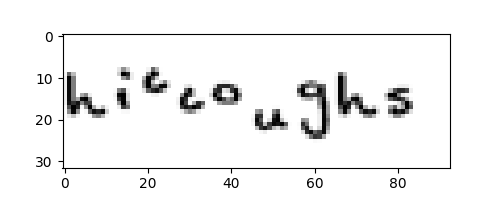
\includegraphics[width=\linewidth]{images/generated_image.png}
    \caption{Generated image using handwritten-like fonts}
    \label{fig:generated_image}
\end{figure}

\subsection{Implementation}



\section{Results \& Discussion}
\label{section:result-discussion}

\subsection{Region of Interest Detection}

It is desirable for ROI detection to cut out the region which is focused by
the user. For example, when a user is writing a sentence,ROI should be a word
written, and when a user is drawing an illustration, ROI should be the whole
illustration drawn.

Since it is difficult to quantitatively measure the goodness of the ROI detection,
only qualitative evaluation was performed this time.
When cutting out only the words that the user is writing in the text,
ROI detection worked almost without failure (Fig \ref{fig:cutting-word-region}).

\begin{figure}
    \centering
    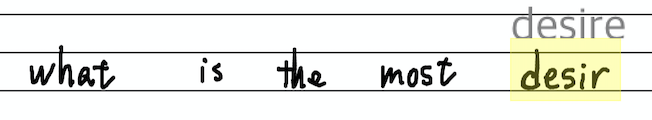
\includegraphics[scale=0.6]{images/word_region.png}
    \caption{ROI detection works well when cutting out a word which is being written}
    \label{fig:cutting-word-region}
\end{figure}

On the other hand, when cutting out a handwritten illustration,
only a part of the illustration may be cut out if the lines constituting
the illustration are not spatially close to each other (Fig \ref{fig:failure}).
Note that the failure example may seem spatially close inside, but it is not the
case when we split it up into a set of strokes and compare the distance between
starting point and ending point of strokes.

\begin{figure}
    \centering
    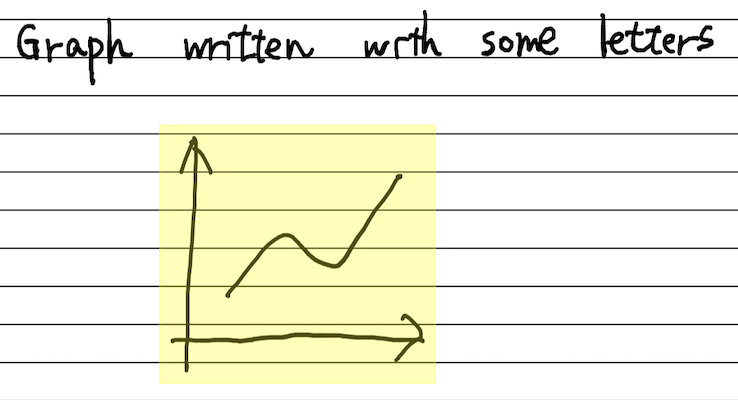
\includegraphics[scale=0.4]{images/illustration.png}
    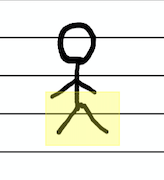
\includegraphics[scale=0.9]{images/failure.png}
    \caption{Left: example of the case ROI detection worked well on illustration. Right: example of failure case of ROI detection}
    \label{fig:failure}
\end{figure}

\subsection{Evaluation of Text recognition}
In the previous section, two patterns of text recognition were tried: recognition using
CTC and recognition using VNRecognizeText API. Since this report worked on recognition of
handwritten text and made use of the result for auto-complete, following metrics were
designed to measure the goodness of auto-completion.

\begin{itemize}
    \item Omitted Characters Count (OCC) - The gap between how many characters did the writer actually write before
    he found the word he wanted to write within top 10 of the auto-completion candidates
    and the number of characters in the word.
    If it is not found after writing to the end, the score is 0. Higher value of this metric indicates better result.
    \item Cumulative Time for Inference (CTI) - Cumulative time spent on auto-completion until the word that the writer actually
    wants to write is included in the top 10 auto-completion candidates. If it is not found after writing to the end,
    the score cumulative time spent on the recognition at each step. Note that each time writer releases the pen tip from the tablet, recognition
    process runs. Lower value of this metric indicates better result.
\end{itemize}

100 words were randomly selected from the word list of `wamerican` package of Debian GNU/Linux for evaluation.
The selected word list is in the repository.
Table \ref{tab:metrics} shows the performance of both methods on auto-completion. While OCC measure of
VNRecognizeText API show better result than CTC, cumulative time elapsed for inference is almost doubled
compared to that of CTC's.

\begin{table}[htbp]
    \centering
    \begin{tabular}{|l||c|c|} \hline
    method & OCC (mean) & CTI (mean) \\ \hline \hline
    CTC & 1.0102 & 1.1060 \\ \hline
    VNRecognizeText (.accurate) & 3.3405 & 1.9751 \\ \hline
    \end{tabular}
    \caption{Perfromance of CTC and VNRecognizeText API on auto-completion.}
    \label{tab:metrics}
\end{table}

\begin{figure}
    \centering
    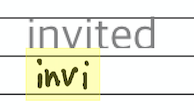
\includegraphics[]{images/auto-completion.png}
    \caption{Example of auto-completion showing the top 1 candidate}
    \label{fig:auto-complete}
\end{figure}

Figure \ref{fig:auto-complete} show an example of how auto-completion works.

\subsection{Discussion}

The VNRecognizeText API is superior to CTC in character recognition accuracy,
but in terms of speed it takes about three times longer to infer.
Since auto-completion is an application that requires real-time performance,
a small lag does not provide a good user experience. Therefore,
poor performance in speed can be a problem.

On the other hand, the CTC model shows inference speed that does not the user
feel uncomfortable in actual use, but the inference result is unstable,
and a slight difference in notation greatly affects the inference result.
Figure \ref{fig:unstable} shows an example of unstable inference.

\begin{figure}
    \centering
    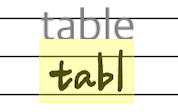
\includegraphics{images/table.png}
    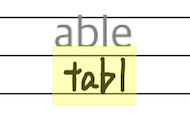
\includegraphics{images/able.png}
    \caption{Example of unstable inference}
    \label{fig:unstable}
\end{figure}

This is probably because training of the CTC model seems to be over-fitty
and strongly depends on the dataset used for training.
Therefore, future tasks include reducing the reliance on datasets and
using larger datasets or using data augmentation techniques to improve generalization performance.

\section{Future Work \& Conclusion}
\label{section:conclusion}

The goal of this report is to create an application to recognize sentences
on iOS for documents where handwritten illustrations and characters were mixed.
Although it is imperfect, the heuristic used for region of interest detection successfully
detect a word out of a sentence, and can cut handwritten illustration out from the other
part of document without requreing large amount of computation.
On the other hand, text recognition had a trade-off between speed and accuracy.

Future tasks include improving the accuracy of text recognition without slowing it down.
Another example of future work is to perform more accurate text recognition and ROI detection
using an online method. In auto-completion, prediction using information on surrounding words,
and refinement of the method of presenting complement candidates can also be one of future works.


\bibliographystyle{IEEEtran}
\bibliography{references}

\end{document}
